\documentclass[a4paper,10pt]{article}
\usepackage[utf8]{inputenc}
\usepackage{hyperref}
\usepackage{multirow}
\usepackage{diagbox}
\usepackage{graphicx}
\usepackage{changepage}
%opening
\title{Classic Concurrency Problem Analysis Report}
\author{Chang Gong - V00898803}
\date{October 11 2018}

\begin{document}

\maketitle

\section{Introduction}
This Report presents an analysis of six classic concurrency problems (5 of them from 'Little Book of Semaphore).The analysis of each problem is divided into three parts: 1.background, 2.evaluation strategy, 3.comparative analysis of  two implementations.The last problem is a concurrency problem of my own.\\

\noindent Tools : Use Java Library Function to measure the performance of Java Program.
Use Go Library and 'StackImpact' to measure the performance of Go routine.\\
All data are averages from five data points.\\


\noindent All code for these implementations can be found \href{https://github.com/MikasaG/CSC-464}{here}. \newline

\section{Readers-Writers Problem}
\subsection{Problem Background}
In computer science, the readers-writers problems are examples of a common computing problem in concurrency. There are at least three variations of the problems, which deal with situations in which many threads try to access the same shared resource at one time. Some threads may read and some may write, with the constraint that no process may access the shared resource for either reading or writing while another process is in the act of writing to it.It pertains to any situation where a data structure, database, or file system is read and modified by concurrent threads. While the data structure is being written or modified it is often necessary to bar other threads from reading, in order to prevent a reader from interrupting a modification in progress and reading inconsistent or invalid data.

This problem is described \href{http://greenteapress.com/semaphores/LittleBookOfSemaphores.pdf#section.4.2}{here}.

\subsection{Evaluation}
I've implemented two implementation of this problem, one is based on fair priority (i.e. read thread and write thread have same priority), another is based on writer-priority algorithm (i.e. no reader can read the resource if there is a writer waiting for writing). Both implementation stemmed from the 'Little Book of Semaphore'. Since I want to investigate the performance difference between these two algorithm instead of different programming language, I implement them by Java.

Same reading and writing tasks are given to these two program (10,000 readings and 100 writings). Some code are written to record the total time each program cost, the average waiting time and longest waiting time for reader and writer threads. The raw results are shown on the table below.

\begin{table}[h]
\centering
\begin{tabular}{ |l|c|c| }
\hline
 \multirow{2}{*}{}&\multicolumn{2}{c|}{\textbf{Implementation}} \\ \cline{2-3}
 & \textbf{Fair Priority} & \textbf{Writer Priority} \\ \hline
\multirow{3}{*}{Average Waiting Time}
 & & \\
 & 1233 ms & 1339 ms \\
  & & \\

\hline
\multirow{3}{*}{Longest Waiting Time}
 & & \\
 & 2009 ms & 2108 ms \\
  & & \\
 \hline

\end{tabular}
\caption{Reader Threads Analysis}
\end{table}


\begin{table}[h]
\centering
\begin{tabular}{ |l|c|c| }
\hline
 \multirow{2}{*}{}&\multicolumn{2}{c|}{\textbf{Implementation}} \\ \cline{2-3}
 & \textbf{Fair Priority} & \textbf{Writer Priority} \\ \hline
\multirow{3}{*}{Average Waiting Time}
 & & \\
 & 2409 ms & 785 ms \\
  & & \\

\hline
\multirow{3}{*}{Longest Waiting Time}
 & & \\
 & 2760 ms & 1757 ms \\
  & & \\
 \hline

\end{tabular}
\caption{Writer Threads Analysis}
\end{table}

\begin{table}[h]
\centering
\begin{tabular}{ |l|c|c| }
\hline
 \multirow{2}{*}{}&\multicolumn{2}{c|}{\textbf{Implementation}} \\ \cline{2-3}
 & \textbf{Fair Priority} & \textbf{Writer Priority} \\ \hline
\multirow{3}{*}{Total Time Cost}
 & & \\
 & 2991 ms & 2472 ms \\
  & & \\

 \hline

\end{tabular}
\caption{Total Time Cost}
\end{table}

\clearpage
\subsection{Compare and Contrast}
{%
\newcommand{\mc}[3]{\multicolumn{#1}{#2}{#3}}
\begin{table}[h]
    \centering
    \begin{adjustwidth}{-3cm}{}
    \setlength{\tabcolsep}{7mm}{
    \begin{tabular}{|p{2.7cm}|p{5.7cm}|p{5.7cm}|} \hline
         \multirow{2}{*}{}&\multicolumn{2}{c|}{\textbf{Implementation}} \\ \cline{2-3}
 & \textbf{Fair Priority} & \textbf{Writer Priority}\\ \hline
        \textbf{Correctness} & From my perspective,Both of the two implementations are correct since they all solve the problem within the restrictions of: 1.Any number of readers can be in the critical section simultaneously. 2.Writers must have exclusive access to the critical section. In the implementation of Fair Priority, readers and writers compete for the resources with the same level of priority, which means a writer could be starved if there are too many readers trying to read the resources. In that case, readers may read unupdated resources consistently& In writer priority implementation, no readers can enter their critical section if there is a writer trying to write, This approach ensures that resources are updated in a timely manner and avoid readers reading stale resources. \\ \hline
        \textbf{Comprehensibility} & Very straight forward and simple, using a mutual lock to protect the critical section of each thread, using a semaphore to indicate whether there are any threads are working, for writers to enter safely &1. A little bit tricky than the previous implementation, it created a structure named 'LightSwith' to help writer thread to prohibit prospective readers entering their critical section. 2.The rest of the code is easy to understand, the thread is basically getting permit from two semaphores then starting its own work.\\ \hline 
         \textbf{Performance} & The fair implementation tends to have a higher overall processing time and average thread wait time, and higher maximum value. It shows a worse performance in all there aspects, especially for the writing threads, a writer could wait over 2.7s, this can be regard as a some sort of starvation.& The Writer Priority implementation got better performance, For readers threads, there was no significant difference, but for writer threads, they only need to wait for 785 ms in average, this is one third of Fair implementation\\ \hline 
    \end{tabular}}
    \end{adjustwidth}
    \caption{Reader-Writer Problem Compare and Contrast}
\end{table}
}%




\newpage
\section{Building H$_2$O}
\subsection{Problem Background}
This problem reflect a common model in many systems, an action require several specific threads to reach a specific point and  cooperate with each other. The natural idea is to construct a reusable barrier to solve this problem, which is exactly what I used in my java implementation. However, using channel is much easier to solve this problem.

This problem is described \href{http://greenteapress.com/semaphores/LittleBookOfSemaphores.pdf#section.5.6}{here}.
\subsection{Evaluation}
I've implemented two implementation of this problem, one is based on Java, using a reusable barrier to help three threads (2 for Hydrogen, 1 for Oxygen) keep same pace before and after they bond as a water molecule. Another implementation is based on Go channel, in such case, threads communication becomes easier and they no longer need a barrier to help them confirm whether they should wait a while for other atom thread. I construct two implementations by two programing language and two completely different threads communication mechinisms, in order to investigate the performance between Java semaphore and Go channel.
Same tasks are given to these two program (30,000 atoms bond to form 10,000 water molecules). Some code are written to record the total time and memory each program cost, I also used 'StackImpact' to measure the performance of Go routine.The raw results are shown on the table below.\\

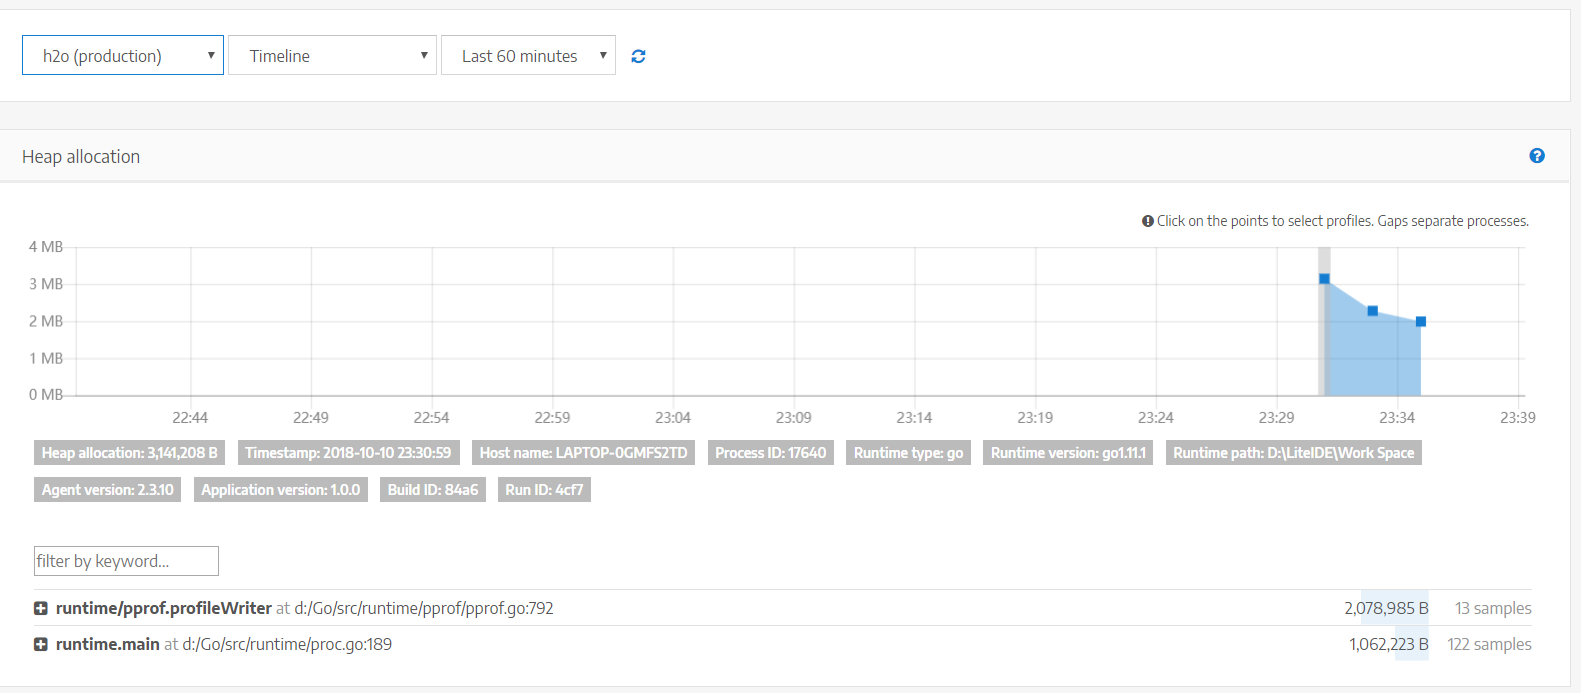
\includegraphics[width=\textwidth]{h2oMemory.PNG}\\

\begin{table}[h]
    \centering
    \begin{tabular}{|c|c|c|c|}
    \hline
        \textbf{Language} & \textbf{Time}& \textbf{Memory Usage}& \textbf{CPU Usage}\\\hline
        Go & 19.9756 ms& 3.00 MB & 0.02\% \\\hline
        Java (Reusable Barrier) & 3807 m & 1089.076 MB& -\\\hline
        
    \end{tabular}
    \caption{Time Cost to form 10,000 water molecules}
\end{table}



\clearpage
\subsection{Compare and Contrast}
{%
\newcommand{\mc}[3]{\multicolumn{#1}{#2}{#3}}
\begin{table}[h]
    \centering
    \begin{adjustwidth}{-3cm}{}
    \setlength{\tabcolsep}{7mm}{
    \begin{tabular}{|p{2.7cm}|p{5.7cm}|p{5.7cm}|} \hline
         \multirow{2}{*}{}&\multicolumn{2}{c|}{\textbf{Implementation}} \\ \cline{2-3}
 & \textbf{Java with Reusable Barrier} & \textbf{Go}\\ \hline
        \textbf{Correctness} & The java implementation is a truly correct way to solve this problem, It creates 30,000 threads to represent 30,000 atoms  and followed the constraints of the problem strictly. If an oxygen or hydrogen thread arrives at the barrier when no partner threads are present, it has to wait for other threads. Only after the previous  water molecule passes through the barrier can the next atoms to bond.& The Go implementation can also be considered as right, Though it using only one thread to imitate the process of constantly creating atoms instead of creating a thread for each atom, it still abides by the rule that only after the previous water molecule gone can the next atoms to bond. Of course, there is no doubt that just starting a thread might give it a performance advantage\\ \hline
        \textbf{Comprehensibility} & Might be hard to understand the code at first, especially for someone who has no knowledge of barrier. A reusable barrier contains two phases, phase 1 make sure every atom are  ready for bonding, phase 2 confirms that every atom finished bonding and ready to leave, It also used one mutual lock and two semaphores to help organize threads.& The Go implementation is easy to understand, comparing to the Java implementation, there are two threads in the program, one for creating Oxygen and Hydrogen atoms randomly, one for receiving these atoms and bond them to form water.\\ \hline
        \textbf{Performance} & There is a pretty substantial difference in the processing time and memory usage, Java implementation cost over 3.8 second and 1089 MB memory to form 10,000 water molecule. I think the big difference in performance caused by the way that Java were used. In Java implementation, it need to start 30,000 threads to solve this problem. & Go program only cost 19.9756ms and 3 MB memory to form 10,000 water mole cute, Go wasn't forced to create a thread for each atom. By make full use of channel mechanism, it only need one thread to imitate the process of generating oxygen and hydrogen atoms. In this problem, Go channel is an absolute efficient choice with huge advantage, comparing to Java Barrier implementation.\\ \hline 
    \end{tabular}}
    \end{adjustwidth}
    \caption{Building H$_2$O Problem Compare and Contrast}
\end{table}
}%

\newpage
\section{Cigarette Smokers Problem}
\subsection{Problem BackGround}
This problem shows up commonly in operating system process scheduling. The agent represents an operating system that allocates resources, and the smokers represent processes that need resources. Resources are available to the processes at different times, each process requires a specific set of resources. The problem is to make sure that if resources are available that would allow one more process to proceed, those processes should be woken up, and avoid waking an process if it cannot proceed.


This problem is described \href{http://greenteapress.com/semaphores/LittleBookOfSemaphores.pdf#section.4.5}{here}.

\subsection{Evaluation}
I've implemented two implementation of this problem, one is based on Java, using three agent threads, three smoker threads to represent agents and smokers, and I used three 'Pusher' threads  that respond to the signals from the agent, keep track of the available ingredients, and signal the appropriate smoker. This idea is stemmed from 'The little book of semaphore'. So in my Java program, there are 9 threads run concurrently. However, in the Go implementation, since the convenience of channel communication, I only need to execute two thread, one imitate the agent and put different ingredients on table constantly, one imitate smokers that looking at the table and decide which kind of smoker should make cigarette now.
Same tasks are given to these two program (10,000 cigarettes). Some code are written to record the total time and memory each program cost, I also used 'StackImpact' to measure the performance of Go routine.The raw results are shown on the table below.\\
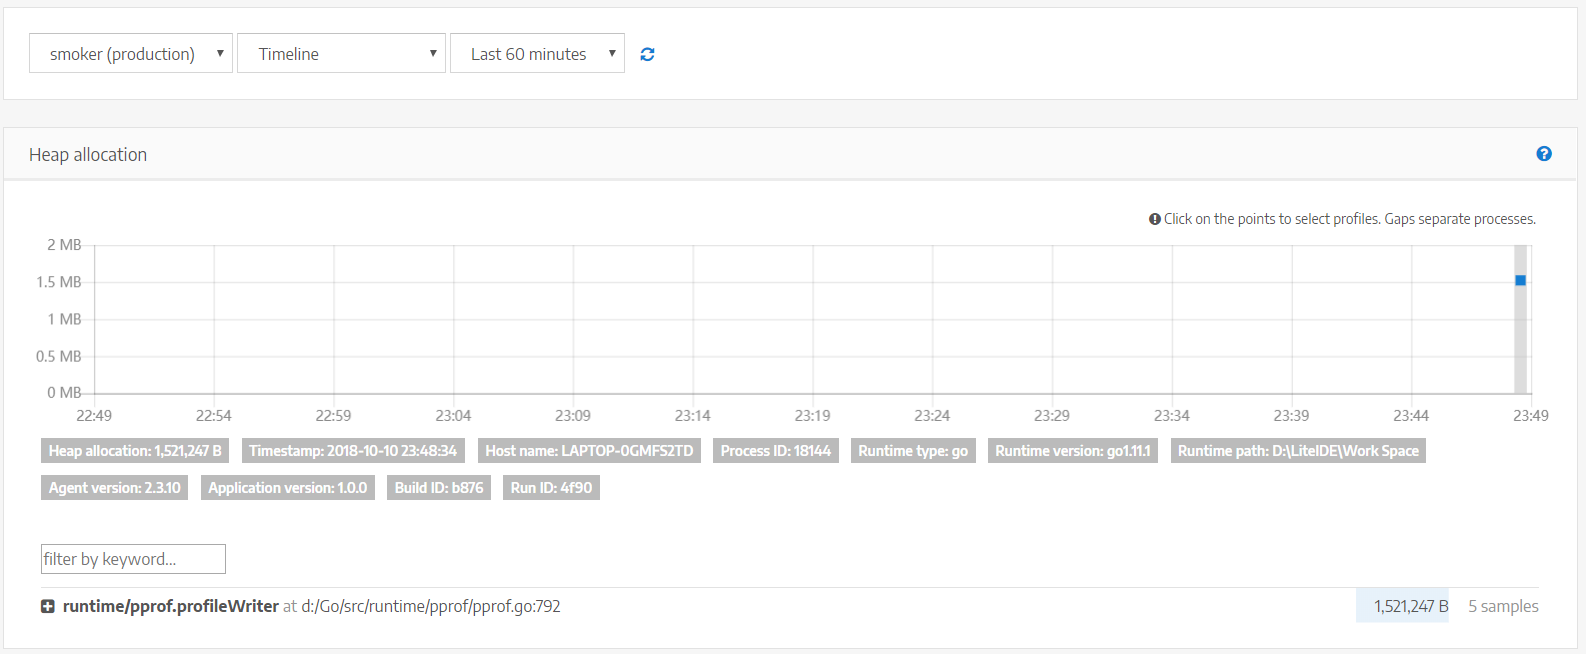
\includegraphics[width=\textwidth]{cigaretteMemory.PNG}\\
\begin{table}[h]
    \centering
    \begin{tabular}{|c|c|c|c|}
    \hline
        \textbf{Language} & \textbf{Time}& \textbf{Memory Usage}& \textbf{CPU Usage}\\\hline
        Go & 36.902 ms & 1.451 MB& 0.01\%\\\hline
        Java (Pusher threads) & 338 ms & 15.379 MB & -\\\hline
    \end{tabular}
    \caption{Time Cost to make 10,000 cigarettes}
\end{table}

\clearpage
\subsection{Compare and Contrast}
{%
\newcommand{\mc}[3]{\multicolumn{#1}{#2}{#3}}
\begin{table}[!htbp]
    \centering
    \begin{adjustwidth}{-3cm}{}
    \setlength{\tabcolsep}{7mm}{
    \begin{tabular}{|p{2.7cm}|p{5.7cm}|p{5.7cm}|} \hline
         \multirow{2}{*}{}&\multicolumn{2}{c|}{\textbf{Implementation}} \\ \cline{2-3}
 & \textbf{Java with Pusher Threads} & \textbf{Go}\\ \hline
        \textbf{Correctness} & The java implementation is absolutely a correct solution since it strictly follow the solution described on the book. It creates 9 threads to represents agents,smokers, and pushers,  and followed the constraints of the problem strictly, that is, each smoker needs a specific set of resources, which cannot be consumed by other smoker at the same time. The creatively use of Pusher threads avoid two smokers hold a resource that each other wants (i.e. dead lock)& The Go implementation can also be considered as right, Though it using only one thread to imitate the smokers to constantly checking the resources on the table instead of creating three threads to represents three smokers, it still abides by the rule that the resources set cannot be consumed by other smoker who cannot smoking at that time. Of course, there is no doubt that just starting a thread might give it a performance advantage\\ \hline
        \textbf{Comprehensibility} & It might cost a code reviewer a while to figure out what does the pusher do, and why pusher threads are necessary, if the comments are not clear. Beside the pusher thread, the rest code are straight forward, three smoker threads and three agent threads are easy to understand, combining the background of the problem& The Go implementation is easier to understand, comparing to the Java implementation, there are two threads in the program, agent thread putting ingredients and pass them to smoker threads through channel, smoker threads constantly checking the resources from channel and decide which kind smoker should smoke now. The use of channel makes it easier to understand the process of passing ingredients.\\ \hline
        \textbf{Performance} & There is a pretty substantial difference in the processing time, Java implementation cost over 338 ms  and 15 MB memory to make 10,000 cigarette. Unlike the Building H$_2$O Problem, this Java implementation only start 9 threads to solve this problem. But it still shows a lower performance than the channel mechanism of Go routine & Go Implementation only cost 36.902ms and 1.45 MB memory to make 10,000 cigarette, The performance came from not only the advantage of having fewer threads but the use of channel mechanism, it only need one thread to imitate the smokers behaviours and it does not need helper thread (Pusher). Comparing to other general synchronization primitive, the performance and usability of Go channel are impressive \\ \hline 
    \end{tabular}}
    \end{adjustwidth}
    \caption{Cigarette Smokers Problem Compare and Contrast}
\end{table}
}%


\newpage
\section{Dining Savages Problem}
\subsection{Problem Background}
This problem reflect a common situation when a set of processes line up for a specific resource (and do their task). A supervisor is responsible for constantly replenishing this resource. The problem is, how to let every general process has the ability to remind the supervisor that it's time for replenishing, and other threads must wait until the resource are available again.

This problem is described \href{http://greenteapress.com/semaphores/LittleBookOfSemaphores.pdf#section.5.1}{here}.
\subsection{Evaluation}
I've implemented two implementation of this problem, one is based on Java, using one Cook thread which running in a loop forever, it constantly check whether there are any savage call him to refill the pot. another thread was used to imitate the process of savages lining up for getting servings. The Go implementation is similar to this, two threads, one for cook, one imitate savages behaviour. The only difference is that the savage used channel to communicate with Cook. Both Java and Go implementation using for loop to imitate savages' line up situation.The intention was to write identical code in both languages, and compare the syntax and performance as such.
Same tasks are given to these two program (1,000,000 savages getting servings from a pot of size 10). Some code are written to record the total time and memory each program cost, I also used 'StackImpact' to measure the performance of Go routine.The raw results are shown on the table below.\\
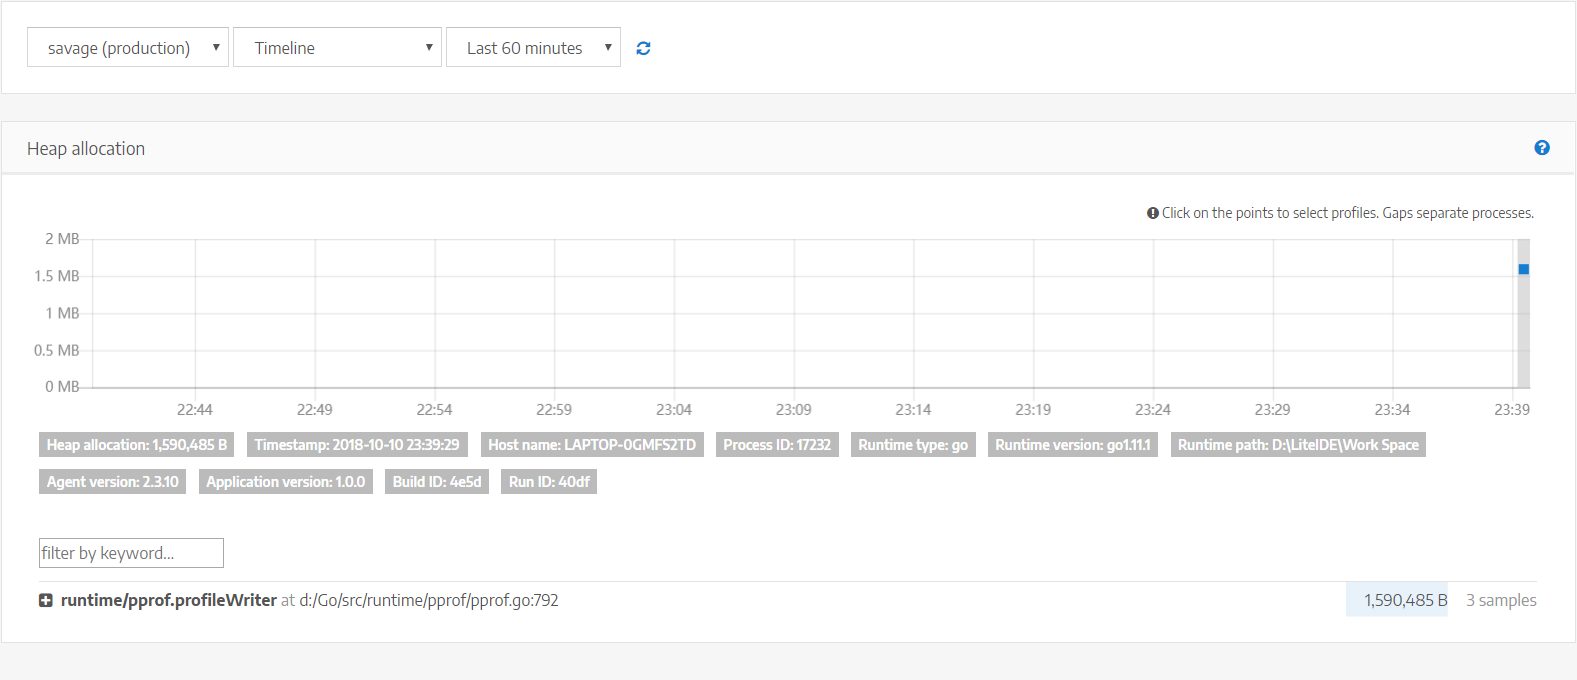
\includegraphics[width=\textwidth]{savageMemmory.PNG}\\
\begin{table}[h]
    \centering
    \begin{tabular}{|c|c|c|c|}
    \hline
        \textbf{Language} & \textbf{Time}& \textbf{Memory Usage}& \textbf{CPU Usage}\\\hline
        Go & 30.3867 sec & 1.520 MB & 0.03\%\\\hline
        Java & 9.132 sec & 49.376 MB & -\\\hline
    \end{tabular}
    \caption{Time Cost for 1,000,000 savages getting servings}
\end{table}

\clearpage
\subsection{Compare and Contrast}
{%
\newcommand{\mc}[3]{\multicolumn{#1}{#2}{#3}}
\begin{table}[!htbp]
    \centering
    \begin{adjustwidth}{-3cm}{}
    \setlength{\tabcolsep}{7mm}{
    \begin{tabular}{|p{2.7cm}|p{5.7cm}|p{5.7cm}|} \hline
         \multirow{2}{*}{}&\multicolumn{2}{c|}{\textbf{Implementation}} \\ \cline{2-3}
 & \textbf{Java} & \textbf{Go}\\ \hline
        \textbf{Correctness} & From my perspectives, both Java and Go solution are correct, since they used almost same algorithms to solve this problem and followed the constrains of it.The reason I used one thread to imitate the situation of savages line up for food, instead of create a thread for every savage is based on the following considerations: In this problem, only one savage can check the pot at a time, Even if implement multiple threads for savage activity, The result is also like a sequential execution & The Go implementation using same algorithm of Java, also using for loop to imitate the savages behaviours, its  correctness is the same as Java implementation\\ \hline
        \textbf{Comprehensibility} & Both Java and Go implementation are very readable, Java use global variables for the synchronization primitives for simplicity. It start two thread to solve the problem nicely.Overall, the code is clean and short and easy to read& The code style in Go implementation is similar to Java , however, it used channel instead of general synchronization primitives, which might the code more comprehensible.\\ \hline
        \textbf{Performance} & The performance of java program surprised me a little bit, Considering that the code between the two languages was practically identical. Java implementation cost only 9 second. This probably because the optimization of JVM for 'for loop', comparing to Go language, however it cost 49 MB memory, I think this is due to language features. Java tend to uses more memory& Go Implementation cost over 30 second to make 1,000,000 savages get their servings. This result indicates that although the go channel has a high performance in the communication activity of a large number of threads, its 'for loop' performance may be much worse than Java\\ \hline 
    \end{tabular}}
    \end{adjustwidth}
    \caption{Dining Savages Problem Compare and Contrast}
\end{table}
}%

\newpage
\section{The Barbershop Problem}
\subsection{Problem Background}
This problem represents a situation where A certain number of applications/processes are allowed to wait for some resource/service. If the number of waiting applications exceeds the maximum value, the subsequent applications will be rejected immediately. The problem is, how a process tell whether it can wait or should be reject, when the service provider know nothing about all these limitation.


This problem is described \href{http://greenteapress.com/semaphores/LittleBookOfSemaphores.pdf#section.5.2}{here}.

\subsection{Evaluation}
I've implemented two implementation of this problem, one is based on Java, using one Barber thread which running in a loop forever and 10,000 customer threads. Every 10ms, a customer thread would start and check whether it can squeeze into the barber's waiting room. However, barber need 15 ms to cut a customer's hair, so some customers would leave barber shop without entering in. The Go implementation is similar to this, one Barber thread and 10,000 Customers routine. It use same time criteria as Java, The only difference is that the Customer used channel to communicate with Barber.The intention was to write identical code in both languages, and compare the syntax and performance as such .

Same tasks are given to these two program (10,000 Customers totally, a customer arrive every 10 ms, barber need 15ms to serve one customer). Some code are written to record the total time and memory each program cost, I also used 'StackImpact' to measure the performance of Go routine.The raw results are shown on the table below.\\
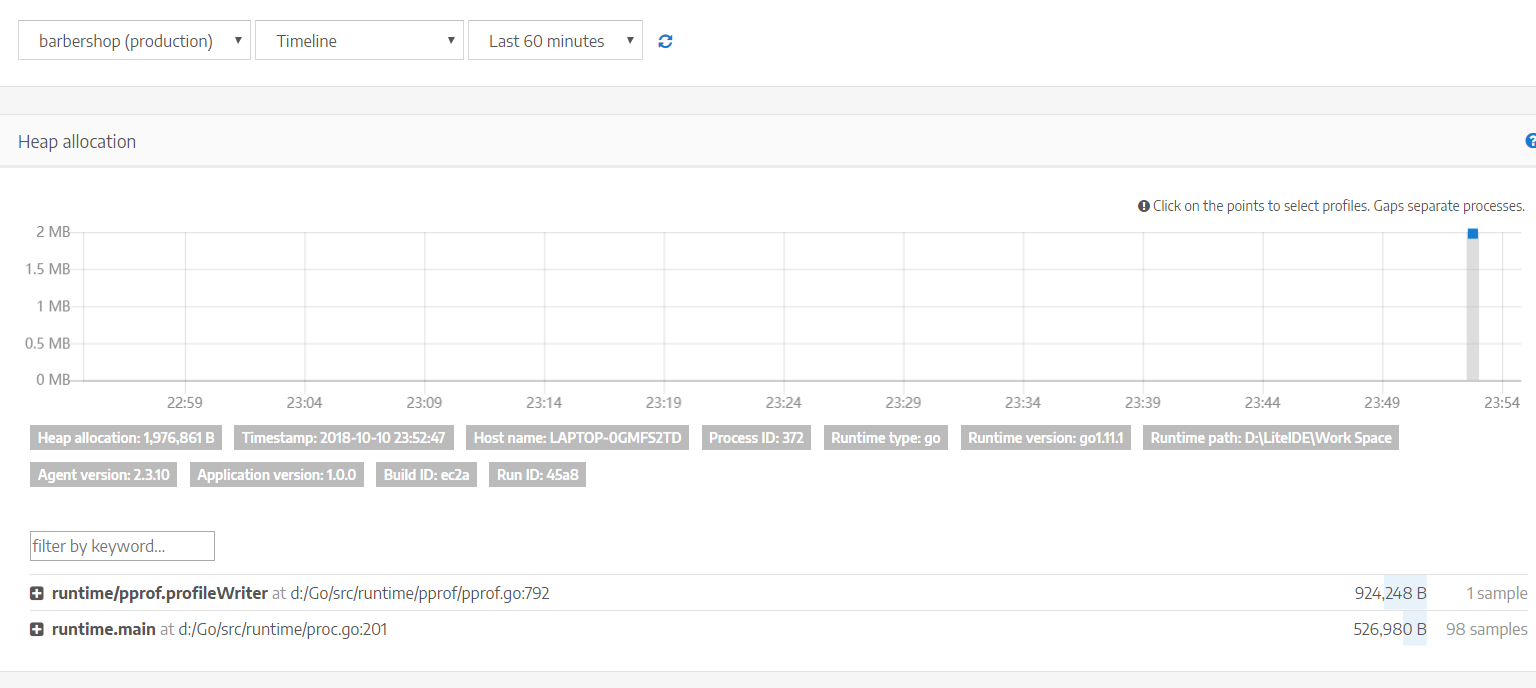
\includegraphics[width=\textwidth]{barberMemory.PNG}\\
\begin{table}[h]
    \centering
    \begin{tabular}{|c|c|c|c|}
    \hline
        \textbf{Language} & \textbf{Time}& \textbf{Memory Usage}& \textbf{CPU Usage}\\\hline
        Go & 108.889 sec & 1.394 MB & 0.02\%\\\hline
        Java & 108.512 sec & 9.396 MB & -\\\hline
    \end{tabular}
    \caption{10,000 Customers totally, customer arrival gap: 10ms, Hair-cut cost: 15ms}
\end{table}

\clearpage
\subsection{Compare and Contrast}
{%
\newcommand{\mc}[3]{\multicolumn{#1}{#2}{#3}}
\begin{table}[!htbp]
    \centering
    \begin{adjustwidth}{-3cm}{}
    \setlength{\tabcolsep}{7mm}{
    \begin{tabular}{|p{2.7cm}|p{5.7cm}|p{5.7cm}|} \hline
         \multirow{2}{*}{}&\multicolumn{2}{c|}{\textbf{Implementation}} \\ \cline{2-3}
 & \textbf{Java} & \textbf{Go}\\ \hline
        \textbf{Correctness} & Both Java and Go solution can be considered as correct, they used almost same algorithms which is stemmed from 'The little book of semaphore', and followed the constrains of it. That is, if the number of waiting customers exceeds the maximum value, the subsequent customers will  leave immediately. I set the time criteria such that every 10ms a customer thread start, but it would cost 15ms for a customer to get hair cut, in order to show the truth that some customers have to leave because the barbershop is full when they arrive. & The Go implementation using same algorithm of Java, also used same time criteria, but it use channel for a customer and barber communicate with each other, so I can investigate the performance differences of two language\\ \hline
        \textbf{Comprehensibility} & Java implementation is readable, There are two kinds of threads, Barber and Customers. The use of four semaphore and one mutual lock may cause comprehensive problem, but I tried to use a clear semaphore name so the functionality of each semaphore can easily tell by its name. The rest code has a clean style, really short and easy to read& The code style in Go implementation is similar to Java , however, it used channel instead of general synchronization primitives, which might the code more comprehensible.\\ \hline
        \textbf{Performance} & There are not much difference between the peroformance of two implementation, Considering that the code between the two languages was practically identical.  Both Java and Go implementaion cost more than 100 second to get 10,000 customers pass through.I think this result was largely caused by the truth that not all customers threads starting at the beginning, one customer thread starts every 15 ms instead, so the thread start time might be the main factor of the program time cost& Go Implementation has a similar performance to java, that might comes from the truth that not all customers threads starting at the beginning, one customer thread starts every 15 ms instead, so the thread start time might be the main factor of the program time cost\\ \hline 
    \end{tabular}}
    \end{adjustwidth}
    \caption{Barber Shop Problem Compare and Contrast}
\end{table}
}%
\newpage
\section{My Own Problem (Matrix Multiplier)}
\subsection{Problem Background}
Matrix multiplication is a simple, classic math problem, Matrix multiplication is used in many fields, such as various data analysis or data prediction models. Many people believe that using concurrency techniques can greatly increase the efficiency of matrix multiplication, but is that really the case? What would we sacrifice by using multiple threads to do matrix multiplication?

\subsection{Evaluation}
I've implemented two implementation of this problem, both of them based on Java. The first one used linear algorithms to compute the matrix multiplication. The second used a thread pool and tried to compute the same matrix with 2,4,8 threads.The intention was to compare the performance of linear approach and concurrent approach.
Same tasks are given to these two program (i.e. The matrix of 1000,2000, and 4000 dimensions). Some code are written to record the total time and memory each program cost.The raw results are shown on the table below.

\begin{table}[h]
    \centering
    \begin{tabular}{|c|c|c|c|}
    \hline
       \textbf{Matrix Dimensions}&  \textbf{Threads Used} & \textbf{Time}& \textbf{Memory Usage} \\\hline
          1000&    Linear&  0.7085 s &  7.70 MB\\\hline
          2000&    Linear&  5.7798 s  & 31.19 MB \\\hline
        4000&   Linear&   46.4368 s& 125.33 MB \\\hline

    \end{tabular}
    \caption{Result of Linear Algorithm}
\end{table}

\begin{table}[h]
    \centering
    \begin{tabular}{|c|c|c|c|}
    \hline
       \textbf{Matrix Dimensions}&  \textbf{Threads Used} & \textbf{Time}& \textbf{Memory Usage} \\\hline

          1000&    2&   0.3917 s&  11.55 MB\\\hline
          1000&    4&   0.2008 s&  21.68 MB\\\hline
          1000&    8&   0.1599 s& 36.66 MB \\\hline

          2000&    2&   2.7292 s&  45.38 MB\\\hline
          2000&    4&   1.6503 s&  80.72 MB\\\hline
          2000&    8&   1.3224 s& 139.43 MB \\\hline

          4000&    2&   24.5674 s&  181.38 MB\\\hline
          4000&    4&   13.7587 s&  303.51 MB\\\hline
          4000&    8&   11.9054 s&  554.04 MB \\\hline
    \end{tabular}
    \caption{Result of Concurrent Algorithm}
\end{table}

\clearpage
\subsection{Compare and Contrast}
{%
\newcommand{\mc}[3]{\multicolumn{#1}{#2}{#3}}
\begin{table}[!htbp]
    \centering
    \begin{adjustwidth}{-3cm}{}
    \setlength{\tabcolsep}{7mm}{
    \begin{tabular}{|p{2.7cm}|p{5.7cm}|p{5.7cm}|} \hline
         \multirow{2}{*}{}&\multicolumn{2}{c|}{\textbf{Implementation}} \\ \cline{2-3}
 & \textbf{Linear Algorithm} & \textbf{Concurrent Algorithm}\\ \hline
        \textbf{Correctness} & Both linear and concurrent algorithm are correct solution for matrix multiplication.They do almost same computational work, but the concurrent algorithm assigns this work to multiple threads and then aggregates their results.& The reason I implemented two algorithms in same language is I want to reduce the variables as much as possible to make the final performance differences all come from the algorithm itself\\ \hline
        \textbf{Comprehensibility} & The linear algorithm is very simple and straight forward. I didn't use  complex data structures to represent a matrix, just a two-dimensional array to represent it. In terms of matrix  computation, it use a for loop to compute the matrix for each row and column. It only need a little bit of math knowledge for someone to understand the algorithm & The code style in Concurrent version is similar to linear version in terms of matrix representation, but it might be a little hard to read the concurrent part for someone who doesn't have relevant background. I used a thread pool to  generate threads and start them automatically, and aggregate the computation results together.\\ \hline
        \textbf{Performance} & There are a lot of things to say in performance difference. Obviously, the time consumption of using linear algorithm is always the largest, but its memory consumption is relatively smaller than multiple threads solutions. Secondly, as the matrix dimension increases, our time consumption and memory resource consumption increase at a rapid rate & As for concurrent algorithm, I listed the performance of implementations using 2,4,8 threads respectively, when we multiply the number of threads, the memory consumption almost doubled, and the total time cost almost become a  half, but this phenomenon is not so obvious after the number of threads reaches 8, It looks like concurrent techniques has an implicit upper limit on time optimization and memory consumption.\\ \hline 
    \end{tabular}}
    \end{adjustwidth}
    \caption{Matrix Problem Compare and Contrast}
\end{table}
}%



\end{document}